%%%% IEEE v1.8b %%%%

%%%% 1. DOCUMENTCLASS %%%%
\documentclass[conference, compsoc]{IEEEtran}

% Some very useful LaTeX packages include:
% (uncomment the ones you want to load)

\usepackage[nocompress]{cite}
\usepackage[pdftex]{graphicx}
\usepackage{url}
\usepackage{caption}
\usepackage{subcaption}
\usepackage[automake=false]{glossaries}
\usepackage[utf8]{inputenc}

% define IEEEtrans command to include specific files
\newcommand*{\IEEEtrans}{}%

% *** Do not adjust lengths that control margins, column widths, etc. ***
% *** Do not use packages that alter fonts (such as pslatex).         ***
% There should be no need to do such things with IEEEtran.cls V1.6 and later.
% (Unless specifically asked to do so by the journal or conference you plan
% to submit to, of course. )

% correct bad hyphenation here
\hyphenation{op-tical net-works semi-conduc-tor}

% declare the path(s) where your graphic files are
\graphicspath{{\docclass/\docname/img/}{cls/IEEEtran/img/}}
% and their extensions so you won't have to specify these with
% every instance of \includegraphics
\DeclareGraphicsExtensions{.pdf, .jpeg, .png}

%% Document informations

%% Required information is doctitle
%% But you're free to add other custom commands ;)

\newcommand{\doctitle}{A Short Example}
\newcommand{\docauthor}{H. Simpson}
%% Acronyms generated from CSV file acrbdd.csv - 2024-02-02
%% Format: {ref name when called in LaTeX}{short version}{long version}

% A
\newacronym{acl}{ACL}{Access Control List}
\newacronym{aslr}{ASLR}{Address Space Layout Randomization}
\newacronym{aes}{AES}{Advanced Encryption Standard}
\newacronym{apb}{APB}{Advanced Peripheral Bus}
\newacronym{arm}{ARM}{Advanced RISC Machines}
\newacronym{atb}{ATB}{Advanced Trace Bus}
\newacronym{abi}{ABI}{Application Binary Interface}
\newacronym{api}{API}{Application Programming Interface}
\newacronym{asic}{ASIC}{Application-Specific Integrated Circuit}
\newacronym{alu}{ALU}{Arithmetic Logic Unit}
\newacronym{adg}{ADG}{Autonomous Dispatcher Gadget}

% B
\newacronym{bios}{BIOS}{Basic Input/Output System}
\newacronym{bht}{BHT}{Branch History Table}
\newacronym{btb}{BTB}{Branch Table Buffer}
\newacronym{btm}{BTM}{Branch Trace Messaging}

% C
\newacronym{cocotb}{Cocotb}{COroutine based COsimulation TestBench}
\newacronym{cpu}{CPU}{Central Processing Unit}
\newacronym{cdc}{CDC}{Clock Domain Crossing}
\newacronym{cra}{CRA}{Code-reuse attack}
\newacronym{csv}{CSV}{Comma-separated Values}
\newacronym{cli}{CLI}{Command-line Interface}
\newacronym{cisc}{CISC}{Complex Instruction Set Computer}
\newacronym{csr}{CSR}{Control and Status Register}
\newacronym{cfg}{CFG}{Control-flow graph}
\newacronym{cfi}{CFI}{Control-flow integrity}
\newacronym{cti}{CTI}{Cross Trigger Interface}
\newacronym{csrf}{CSRF}{Cross-Site Request Forgery}
\newacronym{xss}{XSS}{Cross-Site Scripting}

% D
\newacronym{dep}{DEP}{Data Execution Prevention}
\newacronym{dm}{DM}{Debug Module}
\newacronym{dut}{DUT}{Design Under Test}
\newacronym{dv}{DV}{Design Verification}
\newacronym{dma}{DMA}{Direct Memory Access}
\newacronym{dram}{DRAM}{Dynamic Random Access Memory}

% E
\newacronym{etrace}{E-Trace}{Efficient Trace}
\newacronym{eice}{EmbeddedICE}{Embedded In-circuit Emulation}
\newacronym{etm}{ETM}{Embedded Trace Macrocell}
\newacronym{elf}{ELF}{Executable and Linkable Format}

% F
\newacronym{fpga}{FPGA}{Field-Programmable Gate Array}
\newacronym{fifo}{FIFO}{First In First Out}
\newacronym{fpu}{FPU}{Floating Point Unit}
\newacronym{fop}{FOP}{Function-Oriented Programming}

% G
\newacronym{gsoc}{GSoC}{Global System on a Chip}
\newacronym{gpu}{GPU}{Graphics Processing Unit}

% H
\newacronym{hdd}{HDD}{Hardware Design Document}
\newacronym{htm}{HTM}{Hardware Thread}
\newacronym{hmac}{HMAC}{Hash-based Message Authentication Code}

% I
\newacronym{io}{I/O}{Inputs/Outputs}
\newacronym{isa}{ISA}{Instruction Set Architecture}
\newacronym{x86}{x86}{Intel's Instruction Set Architecture}
\newacronym{ip}{IP}{Intellectual Property}
\newacronym{iot}{IoT}{Internet of Things}
\newacronym{ids}{IDS}{Intrusion Detection System}
\newacronym{ips}{IPS}{Intrusion Prevention System}

% J
\newacronym{jtag}{JTAG}{Joint Test Action Group}
\newacronym{jop}{JOP}{Jump-Oriented Programming}
\newacronym{jit_rop}{JIT-ROP}{Just-In-Time Return-Oriented Programming}
\newacronym{jit}{JIT}{Just-In-Time compilation}

% L
\newacronym{lbr}{LBR}{Last Branch Record}
\newacronym{lsb}{LSB}{Less Significant Bit}
\newacronym{lop}{LOP}{Loop-Oriented Programming}

% M
\newacronym{cache}{Cache}{Memory Cache}
\newacronym{mmu}{MMU}{Memory Management Unit}
\newacronym{mpu}{MPU}{Memory Protection Unit}
\newacronym{mdo}{MDO}{Message Data Out}
\newacronym{mseo}{MSEO}{Message Start/End Out}
\newacronym{mips}{MIPS}{Microprocessor without Interlocked Pipeline Stages}

% N
\newacronym{noc}{NoC}{Network on Chip}
\newacronym{ntrace}{N-Trace}{Nexus Trace}
\newacronym{nx}{NX}{No-Execute}

% O
\newacronym{os}{OS}{Operating System}

% P
\newacronym{pmp}{PMP}{Physical Memory Protection}
\newacronym{pcb}{PCB}{Printed Circuit Board}
\newacronym{pc}{PC}{Program Counter}
\newacronym{pldrc}{PLDRC}{Progressive Logic Design Rule Checking}
\newacronym{pki}{PKI}{Public Key Infrastructure}

% R
\newacronym{ram}{RAM}{Random Access Memory}
\newacronym{rng}{RNG}{Random Number Generator}
\newacronym{rom}{ROM}{Read-Only Memory}
\newacronym{risc}{RISC}{Reduced Instruction Set Computer}
\newacronym{riscv}{RISC-V}{Reduced Instruction Set Computer "V"}
\newacronym{rtl}{RTL}{Register Transfer Level}
\newacronym{ras}{RAS}{Return Address Stack}
\newacronym{rop}{ROP}{Return-Oriented Programming}
\newacronym{rsa}{RSA}{Rivest-Shamir-Adleman}

% S
\newacronym{sha}{SHA}{Secure Hash Algorithm}
\newacronym{ssl_tls}{SSL/TLS}{Secure Sockets Layer/Transport Layer Security}
\newacronym{scs}{SCS}{Shadow Call Stack}
\newacronym{srop}{SROP}{Sigreturn-Oriented Programming}
\newacronym{sram}{SRAM}{Static Random Access Memory}
\newacronym{soc}{SoC}{System on Chip}

% T
\newacronym{tg}{TG}{Task Group}
\newacronym{tsc}{TSC}{Technical Steering Committee}
\newacronym{te}{TE}{Trace Encoder}
\newacronym{tpm}{TPM}{Trusted Platform Module}

% U
\newacronym{uefi}{UEFI}{Unified Extensible Firmware Interface}
\newacronym{uart}{UART}{Universal Asynchronous Receiver-Transmitter}
\newacronym{uvm}{UVM}{Universal Verification Methodology}

% V
\newacronym{vpn}{VPN}{Virtual Private Network}

% Y
\newacronym{yolo}{YOLO}{You only live once}


\makeglossaries

\begin{document}

% paper title
% Titles are generally capitalized except for words such as a, an, and, as,
% at, but, by, for, in, nor, of, on, or, the, to and up, which are usually
% not capitalized unless they are the first or last word of the title.
% Linebreaks \\ can be used within to get better formatting as desired.
% Do not put math or special symbols in the title.
\title{\doctitle}

% author names and affiliations
% use a multiple column layout for up to three different
% affiliations
\ifdefined\TCHES

\author{Homer Simpson\inst{1} \and al\inst{1}}
\institute{
  Springfield Nuclear Power Plant, Springfield, US \email{homer.simpson@snpp.com}
}

\fi

\ifdefined\IEEEtran

\author{\IEEEauthorblockN{Téo Biton}
\IEEEauthorblockA{Springfield Nuclear\\ Power Plant \\
Springfield, US \\
Email: homer.simpson@snpp.com}}

\fi


% make the title area
\maketitle

% main text of the article
\documentclass[]{article}

%\usepackage[utf8]{inputenc} % encode en UTF8

%\usepackage[T1]{fontenc}
%\usepackage[utf8]{inputenc}
%\usepackage{lmodern}
%\usepackage{babel}

\usepackage[top=2.54cm, bottom=2.54cm, left=3.81cm, right=3.81cm]{geometry}
\usepackage{graphicx}
\usepackage{caption}
\usepackage{subcaption}
\usepackage{xcolor}
\usepackage{float}
\usepackage{soul}

\newcommand{\gap}{\vspace{5mm}}

%Belles fraction de fration \cfrac
%\usepackage{amsmath}

%\usepackage{tikz}
%\usepackage{circuitikz}

\usepackage{listings}             % Include the listings-package
%\lstset{language=Matlab}          % Set your language (you can change the language for each code-block optionally)
%\lstset{language=C}

\usepackage{multicol}
\usepackage{array}
% Gray horizontal lines for tables 
\usepackage{colortbl}
% Space between lines for tables
\usepackage{booktabs}
\newcommand{\rhline}{\midrule[0.1mm]}% \addlinespace[1ex]\arrayrulecolor{gray}\hline\arrayrulecolor{black}\addlinespace[1ex]}

%% User style for C

 \usepackage{color}
% \usepackage{xcolor}

\definecolor{mGreen}{rgb}{0,0.6,0}
\definecolor{mGray}{rgb}{0.5,0.5,0.5}
\definecolor{mPurple}{rgb}{0.58,0,0.82}
\definecolor{backgroundColour}{rgb}{0.95,0.95,0.95}

\lstdefinestyle{CStyle}{
    language=C,
    tabsize=4,
    captionpos=b,
    numbers=left,
    commentstyle=\color{mGreen},
    backgroundcolor=\color{white},
    numberstyle=\color{gray},
    keywordstyle=\color{blue} \textbf,%otherkeywords={xdata},
    keywords=[2]{xdata},
    keywordstyle=[2]\color{red}\textbf,
    identifierstyle=\color{black},
    stringstyle=\color{red}\ttfamily,
    basicstyle = \ttfamily \color{black} \footnotesize,
    inputencoding=utf8/latin1,
    showstringspaces=false,
    frame=single,
    morekeywords={uint32_t, uint16_t, uint8_t, inline, state_t,
    uticks_t, atomic, endatomic, @brief, CTRL_IT_t, ID_IT_t}
}










% the glossary definition needs to be in .sty
% Seems to be because of different directories

\usepackage[
   record,
    acronym,
    %style=longheader,
    % indexonlyfirst,
   % nopostdot
    ]{glossaries-extra}
\setabbreviationstyle[acronym]{long-short} % first occurence long, rest short
%\setabbreviationstyle{long-short} % first occurence long, rest short

%\usepackage[record]{glossaries-extra}
\GlsXtrLoadResources[src={terms}]


 % latex configuration

\begin{document}

\newcommand{\HRule}{\rule{\linewidth}{0.5mm}} % Definition epaisseur des lignes horizontales

\vspace*{1cm}

\begin{center} % title
	\HRule \\[0.2cm] %vertical line
	\Large
	\textbf{
		TITLE
		}\\ %Titre
	\vspace{1cm}
Document topic \\

	\large
	\HRule \\[1.5cm] %vertical line
	\normalsize
	\author{[AUTOR]}
	\today %date
\end{center}

\begin{figure}[h!] %logos
	\centering
	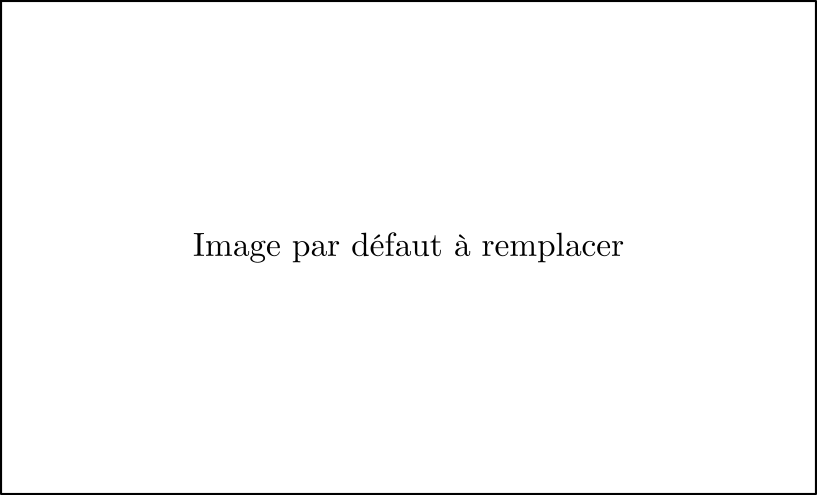
\includegraphics[width=0.6\linewidth]{./img-data/default.png}
\end{figure}

\vspace{2cm}

\begin{center}\large %School
	\textsc{School}\\
	\textsc{Option}
\end{center}

\vspace{2cm}

\noindent
Enseignant référent : 
\vspace{2cm}


\newpage

% ----------------------------------------------------------------
% ----------------------- Table of content -----------------------
% ----------------------------------------------------------------

\tableofcontents

\vspace{1cm}
\listoffigures

\vspace{1cm}
\listoftables

% ----------------------------------------------------------------
% ------------------------- Introduction -------------------------
% ----------------------------------------------------------------

\vspace*{4cm}
\section*{Résumé}
La Méthodologie de Conception de Systèmes Electroniques est une discipline essentielle lorsqu'il s'agit, dans le cadre d'une future carrière d'ingénieur, de réaliser un produit répondant aux besoins d'un client.
Et ce domaine est d'autant plus indispensable dans un monde où les systèmes numériques sont de plus en plus complexes et leur conceptions demandent une bonne structuration et une réelle méthodologie.
Ce rapport s'inscrit dans la présentation d'une conception d'un système de lavage de voiture par l'utilisation d'une méthode précise, applicable dans un ensemble de secteurs d'activités comme l'automobile, le médical, l'aéronautique, maritime, que ce soit dans le civil ou le militaire.
Il s'agit de concevoir un système simplifié de pilotage d'un portique de lavage de voiture.
Ainsi, et afin de simplifier l'exercice, on ne considère que le rouleau horizontal du portique.

\newpage

\section{Introduction}

\subsection{Contextualisation}
La formation ETN (Électronique et technologies numériques) offerte par l'école polytechnique de l'Université de Nantes propose d'aborder diverses branches de l'électronique, du traitement du signal au systèmes à microprocesseur en passant par l'électronique analogique des hautes-fréquences.
Cet ensemble de domaines techniques nécessite des compétences en matière de méthodologie de conception. Ce rapport s'inscrit dans la conception d'un appareil de marquage routier avec la méthode MCSE.
La méthode MCSE (Méthode de conception des systèmes électroniques), née à Ireste par l'impulsion de Jean-Paul Calvez, cette méthode a été implantée au sein d'un outil nommée CoFluent rachetée par Intel\mbox{\textregistered } depuis 2011. Cette méthode fait désormais partie de la culture de la formation et constitue l'outil de conception premier de l'ingénieur ETN.\\
Ce rapport se décompose en diverses parties.
Il s'agira dans un premier temps de rappeler le cahier des charges de la conception \hl{.......} %TODO
Pour l'ensemble de ce rapport, les diverses phases de spécifications et conceptions s'appuient sur les deux ouvrages de Jean-Paul Calvez. \cite{Calvez_1} \cite{Calvez_2} \\
Ce travail de conception à pour but de placer les étudiants dans un contexte industriel. Le cahier des charges fourni prend la forme d'un exemple réel où les spécifications du client sont exprimées.


\begin{figure}
    \centering
    \includegraphics[width=\linewidth]{img-data/default_svg.draw.pdf}
\end{figure}



% ----------------------------------------------------------------
% ------------------------- Conclusion ---------------------------
% ----------------------------------------------------------------

\newpage
\section{Conclusion}

Lorem ipsum dolor sit amet, consectetur adipiscing elit, sed do eiusmod tempor incididunt ut labore et dolore magna aliqua. Ut enim ad minim veniam, quis nostrud exercitation ullamco laboris nisi ut aliquip ex ea commodo consequat. Duis aute irure dolor in reprehenderit in voluptate velit esse cillum dolore eu fugiat nulla pariatur. Excepteur sint occaecat cupidatat non proident, sunt in culpa qui officia deserunt mollit anim id est laborum.Lorem ipsum dolor sit amet, consectetur adipiscing elit, sed do eiusmod tempor incididunt ut labore et dolore magna aliqua. Ut enim ad minim veniam, quis nostrud exercitation ullamco laboris nisi ut aliquip ex ea commodo consequat. Duis aute irure dolor in reprehenderit in voluptate velit esse cillum dolore eu fugiat nulla pariatur. Excepteur sint occaecat cupidatat non proident, sunt in culpa qui officia deserunt mollit anim id est laborum.Lorem ipsum dolor sit amet, consectetur adipiscing elit, sed do eiusmod tempor incididunt ut labore et dolore magna aliqua. Ut enim ad minim veniam, quis nostrud exercitation ullamco laboris nisi ut aliquip ex ea commodo consequat. Duis aute irure dolor in reprehenderit in voluptate velit esse cillum dolore eu fugiat nulla pariatur. Excepteur sint occaecat cupidatat non proident, sunt in culpa qui officia deserunt mollit anim id est laborum.Lorem ipsum dolor sit amet, consectetur adipiscing elit, sed do eiusmod tempor incididunt ut labore et dolore magna aliqua. Ut enim ad minim veniam, quis nostrud exercitation ullamco laboris nisi ut aliquip ex ea commodo consequat. Duis aute irure dolor in reprehenderit in voluptate velit esse cillum dolore eu fugiat nulla pariatur. Excepteur sint occaecat cupidatat non proident, sunt in culpa qui officia deserunt mollit anim id est laborum.

% ----------------------------------------------------------------
% ----------------------- Biblio - glossary ----------------------
% ----------------------------------------------------------------

\newpage

% Atleast one acronym must be used, if not the glossary crashes
\gls{CPU}

\printunsrtglossary[type=acronym]

\newpage
% Atleast one citation must be used, if not the biblo crashes
\cite{Calvez_1}
\bibliography{proj_bibli}{}
\bibliographystyle{plain}

% ----------------------------------------------------------------
% -------------------------- Appendix ----------------------------
% ----------------------------------------------------------------

\newpage
\section{Appendix}




\end{document}


% references section
\bibliographystyle{IEEEtran}
\bibliography{cls/IEEEtran/IEEEabrv, common/Bibliography}

% that's all folks
\end{document}